\chapter{C++ Implementation}
%TODO update the content below, migrate commentary, input usage file...

The above transformations have been implemented in C++.  Program \lsti{main} takes one argument specifying the type of input object (V-Cone, V-Polyhedra, H-Cone, or H-Polyhedra).  It reads the description of the object from standard input, and writes the result of the implied transformation to standard output (details below).  If no arguments are supplied, then a \lsti{usage} message is given.  The \lsti{usage} message, which also contains the input format for the objects, is:
\bigskip
\hrule
\VerbatimInput{../../usage.txt}
\hrule

The files pertaining to the implementation will be discussed in the following sections, but here is a table showing the include dependencies followed by a short summary of the files. \\

\begin{tabular}{|l|l|}
	\hline
	file                          & includes                                             \\
	\hline
	\filename{linear\_algebra.h}  & \filename{<C++ standard library>}                    \\
	\filename{fourier\_motzkin.h} & \filename{linear\_algebra.h}                         \\
	\filename{polyhedra.h}        & \filename{fourier\_motzkin.h}                        \\
	\filename{main.cpp}           & \filename{polyhedra.h}                               \\
	\hline
	\filename{test\_functions.h}  & \filename{linear\_alebra.h}                          \\
	\filename{test.cpp}           & \filename{test\_functions.h}, \filename{polyhedra.h} \\
	\hline
\end{tabular}\\

\vspace{1em}

Here is a very brief summary of the files mentioned in the above table, more details are given in subsequent sections.

\begin{itemize}
	\item \texttt{linear\_algebra.h} \\
	      Defines the types \lsti{Vector} and \lsti{Matrix}, which are the primary means of representing polyhedra, and some basic functionality for them
	\item \texttt{fourier\_motzkin.h} \\
	      Implementation of Fourier Motzkin elimination, and the {\MWT} for cones
	\item \texttt{polyhedra.\{cpp,h\} } \\
	      Transforms between cones and polyhedra, completing the {\MWT}
	\item \texttt{test\_functions.h} \\
	      Types and functions for testing the algorithms (see \Cref{chap_testing}).
	\item \texttt{test.cpp} \\
	      Test cases for the algorithms and functions from \filename{test\_functions.h}
\end{itemize}

\section{Code}

The relevant code will be displayed with commentary below.  Some of the code relating to C{++} specific technicalities and I/O is omitted.

\section{\filename{linear\_algebra.h}}
The types \lsti{Vector} and \lsti{Vectors} are used in the representation of polyhedra.  The \lsti{std::valarray} template is used because it has built-in vector-space operations (sum and scaling).  \lsti{std::vector} is used as a container of \lsti{Vector}s, however other containers could be used.
\lsttdVecs

The \lsti{class Matrix} implements a subset of what a \textit{C++ Container} should.  It is the primary type for representing polyhedra, and directly represents Cones, as well as H-Polyhedra.  The class is designed to enforce the following invariant:
\[ (\forall \mli{v} \in \mli{vectors})\, \mli{v.size() == d} \]
The factory function \lsti{read_Matrix} is provided to read a \lsti{Matrix} from an \lsti{istream}.  It is necessary because the value of \lsti{d} can't be known before reading some of the stream.
\lstMatrix

The \lsti{struct VPoly} gather two \lsti{Matrices} needed to represent a V-Polyhedron.  The \lsti{Matrix U} corresponds to the rays that generate the cone, and the \lsti{Matrix V} corresponds to the points, i.e.
\[ \mli{vpoly} = \cone(\mli{vpoly.U}) + \conv(\mli{vpoly.V}) \]
\lstVPoly

The \lsti{class input_error} is thrown to indicate an invalid input to the program, and provide some clue as to why it failed.  Here are two command line examples:
\VerbatimInput{../../bad_usage.txt}

\lstinputerror

\lsti{operator>>} and \lsti{operator<<} implement the input format described in \\\filename{usage.txt}.
\lstissV
\lstossV

\lsti{usage()} outputs the usage message shown above.
\lstusage

\section{\filename{linear\_algebra.cpp}}
\lsti{e_k} creates the canonical basis \lsti{Vector} $\e_k \in \R^d$.
\lstek

\lsti{concatentate} takes the \lsti{Vector}s $\mli{l} \in \R^{\mli{l.size()}}$ and $\mli{r} \in \R^{\mli{r.size()}}$ and \lsti{return}s the \lsti{Vector} $(\mli{l,r}) \in \R^{\mli{l.size() + r.size()}}$
\lstconcatenate

\lsti{get_column} \lsti{return}s the \lsti{k}-th column of the \lsti{Matrix M}.  Note that while a \lsti{Matrix} may logically represent either a collection of row or column \lsti{Vector}s, \lsti{get_column} is only used in the function \lsti{transpose}, where this distinction is unimportant.
\lstgetcolumn

\lsti{transpose} \lsti{return}s the transpose of \lsti{Matrix M}.
\lsttranspose

A \lsti{slice} object can be used to conveniently obtain a subset of a \lsti{valarray}.  \lsti{slice_matrix} \lsti{return}s the \lsti{Matrix} obtained by applying the \lsti{slice s} to each \lsti{Vector} of the \lsti{Matrix}.
\lstslicematrix

\section{\filename{fourier\_motzkin.cpp}}

A \lsti{slice} object is determined by three fields: \lsti{start}, \lsti{size}, and \lsti{stride}, and implicitly represents all indices of the form:
\[ \sum_{0 \leq k < \mli{size}} \mli{start} + k\cdot\mli{stride} \]
Therefore:
\[i \in \mli{slice} \Leftrightarrow
	\begin{cases}
		i - \mli{start} \equiv 0 \mod(\mli{stride}) \\
		\mli{start} \leq i \leq \mli{start} + {\mli{stride}}\cdot\mli{size}
	\end{cases}\]
\lstindexinslice

\lsti{fourier_motzkin} takes a \lsti{Matrix M} and a coordinate \lsti{k} and creates the set which either corresponds to a projection of an H-Cone (without reducing the dimensionality), or the intersection of a V-Cone with a coordinate-hyperplane.
\lstfouriermotzkin

The lines:
\lstFMEPart
Partition \lsti{M} into logical sets $Z,P,N$ that satisfy the following:\\

\begin{tabular}{|l|l|l|}
	\hline
	set & range                               & property     \\
	\hline
	$Z$ & [\lsti{M.begin()}, \lsti{z_end} $)$ &
	\lsti{it} $\in Z \Leftrightarrow$ \lsti{(*it)[k]} $ = 0$ \\
	\hline
	$P$ & [\lsti{z_end}, \lsti{p_end} )       &
	\lsti{it} $\in P \Leftrightarrow$ \lsti{(*it)[k]} $ > 0$ \\
	\hline
	$N$ & [\lsti{p_end}, \lsti{M.end()})      &
	\lsti{it} $\in N \Leftrightarrow$ \lsti{(*it)[k]} $ < 0$ \\
	\hline
\end{tabular}\\

The line:
\lstFMEMove
Moves $Z$ into the result.  The lines:
\lstFMEConvolute
convolute the vectors in the way described in \Nameref{fm_hcone} and \Nameref{fm_vcone} (concerning projecting an H-Cone and intersecting a V-Cone with a coordinate-hyperplane), and push them into the result \lsti{Matrix}.  In particular, it creates the sets which correspond to
\[ \set{\Bik B_j - \Bjk B_i \st i \in P,\, j \in N}, \quad
	\set{\Yi Y^j - \Yj Y^i \st i \in P,\, j\in N} \]

\lsti{sliced_fourier_motzkin} applies \lsti{fourier_motzkin} to \lsti{Matrix M} for each ${k \not\in \mli{s}}$, then slices the resulting \lsti{Matrix} using \lsti{slice_matrix} and \lsti{s}.  This is the realization of the algorithms indicated by the proofs of either direction of the {\MWT} for cones.  (Here, the slice operation is used to reduce the dimensionality as appropriate).
\lstslicedfouriermotzkin

When transforming an H-Cone to a V-Cone, it first must be written as a V-Cone of a new matrix, then it is intersected with coordinate-hyperplanes and projected.  Similarly, when a V-Cone is transformed into an H-Cone, it must be written as and H-Cone of a new matrix then projected with coordinate-projections.  The transformations are described in \nameref{vconelift_transform} and \nameref{hconelift_transform}, and summarized here:
\[\HLift(A) = \pmb \0 & I & -I \\ I & A & -A \pme \quad
	\VLift(U) = \pmb \0 & -I \\ I & -U \\ -I & U \pme \]
Note that the tranformation of $U$ can be written:
\[\VLift(U) = \pmb \0 & I & -I \\ -I & -U & U \pme^T \]

Remembering that a \lsti{Matrix} is either a collection of row \textit{or} column \lsti{Vector}s, it is not surprising that these two transformations can be written as one function whose parameters are a \lsti{Matrix} and some coefficients.  In \lsti{generalized_lift}, the coefficients are given as an \lsti{array<double, 5> C}, so the overall transformation can be illustrated as:
\newcommand{\CA}[1]{\mli{C[#1]}}
\[ \mli{Matrix M} \to
	\begin{pmatrix*}[r]
		\0 & \CA{0}I \\
		\CA{1}I & \CA{2}\mli{M} \\
		\CA{3}I & \CA{4}\mli{M}
	\end{pmatrix*} \]
where \lsti{Matrix M} is a collection of row \lsti{Vector}s, or
\[ \mli{Matrix M} \to
	\begin{pmatrix*}[r]
		\0 & \CA{1}I & \CA{3}I \\
		\CA{0}I & \CA{2}\mli{M} & \CA{4}\mli{M}
	\end{pmatrix*} \]
where \lsti{Matrix M} is a collection of column \lsti{Vector}s.
\lstgeneralizedlift

\lsti{lift_vcone} and \lsti{lift_hcone} implement the appropriate transformation using \lsti{generalized_lift} and providing the appropriate coefficients in \\
\lsti{array<double, 5> C}.
\lstliftvcone
\lstlifthcone

\lsti{cone_transform} consolidates the logic of the V-Cone $\to$ H-Cone and H-Cone $\to$ V-Cone transformations by accepting a \lsti{Matrix cone} and a \lsti{LiftSelector}.  The LiftSelector type is an enumerable class, used to avoid the need for function pointers.
\lstconetransform

\lsti{vcone_to_hcone} and \lsti{hcone_to_vcone} specialize \lsti{cone_transform} by providing the appropriate \lsti{Lift}.
\lstvconetohcone
\lsthconetovcone

\section{\filename{polyhedra.cpp}}

\lsti{hpoly_to_hcone} and \lsti{hcone_to_hpoly} implement the \lsti{Matrix} transforms:
\[ \mli{hpoly_to_hcone}: (A|b) \to (-b|A),\quad \mli{hcone_to_hpoly} : (-b|A) \to (A|b) \]
These very simple transforms are done with the \lsti{cshift} function, which ``circularly shifts'' the elements of a \lsti{Vector} (provided as part of the interface to \lsti{valarray}).
\lsthpolytohcone
\lsthconetohpoly

\lsti{vpoly_to_vcone} implements the \lsti{VPoly} transform:
\[ \mli{vpoly} \to
	\begin{pmatrix}
		\0 & \vec{1} \\ \mli{vpoly.U} & \mli{vpoly.V}
	\end{pmatrix} \]
\lstvpolytovcone

\lsti{normalized_P} takes the members of \texttt{U} that have $x_0 > 0$, scaled by $1/x_0$.  Let $\Pi$ be the identity matrix with the $0$-th row deleted, and $P = \set{\u \in U : u_0 > 0}$. then this is the result of:
\[ \Pi\left(\set{\x/x_0 : \x\in P} \cap \set{x_0 = 1}\right) \]
\lstnormalizedP

\lsti{vcone_to_vpoly} implements \nameref{vcone_to_vpoly}.
\lstvconetovpoly

\lsti{hpoly_to_vpoly} and \lsti{vpoly_to_hpoly} implement the complete transformations promised by the file.
\lsthpolytovpoly
\lstvpolytohpoly

\section{Picture of the Program}
In the following diagram, the nodes represent functions, and the edges can be read as ``calls.''  Such a diagram is known as a ``callgraph,'' and is only intended to give an overview of the program.

For such a small callgraph, observation is enough to get some insight into the program.  In particular, the nodes with the highest degrees (5) are: \\
\texttt{fourier\_motzkin}, \texttt{cone\_transform}, and \texttt{generalized\_lift}.  Each have two incoming edges, reflecting the ``H'' vs ``V'' aspects of the program.  It makes sense that these would be the functions getting higher degree in the program, as these are (roughly speaking) the most important parts of the proof of the theorem.
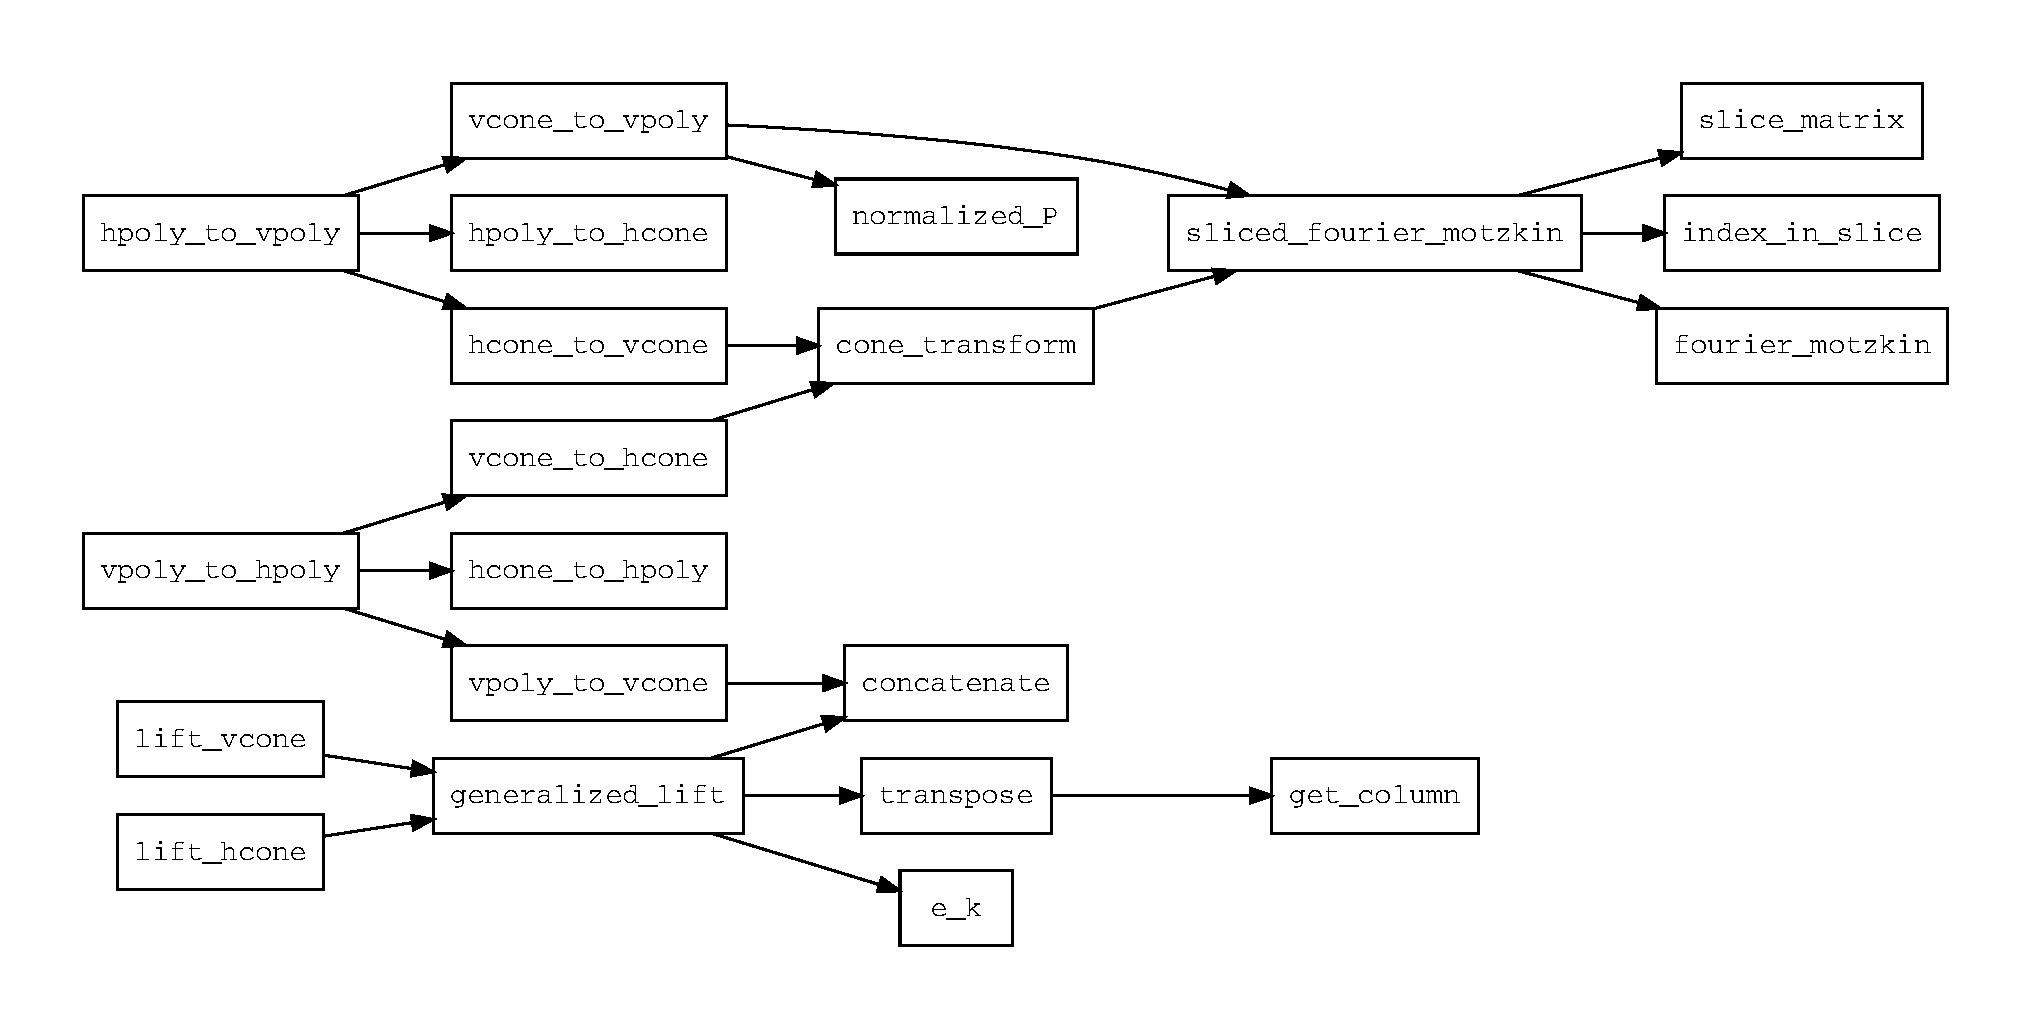
\includegraphics[keepaspectratio,width=\textwidth,height=\textheight]{../img/callgraph.pdf}

